% Options for packages loaded elsewhere
\PassOptionsToPackage{unicode}{hyperref}
\PassOptionsToPackage{hyphens}{url}
\PassOptionsToPackage{dvipsnames,svgnames,x11names}{xcolor}
%
\documentclass[
  letterpaper,
  DIV=11,
  numbers=noendperiod]{scrartcl}

\usepackage{amsmath,amssymb}
\usepackage{iftex}
\ifPDFTeX
  \usepackage[T1]{fontenc}
  \usepackage[utf8]{inputenc}
  \usepackage{textcomp} % provide euro and other symbols
\else % if luatex or xetex
  \usepackage{unicode-math}
  \defaultfontfeatures{Scale=MatchLowercase}
  \defaultfontfeatures[\rmfamily]{Ligatures=TeX,Scale=1}
\fi
\usepackage{lmodern}
\ifPDFTeX\else  
    % xetex/luatex font selection
\fi
% Use upquote if available, for straight quotes in verbatim environments
\IfFileExists{upquote.sty}{\usepackage{upquote}}{}
\IfFileExists{microtype.sty}{% use microtype if available
  \usepackage[]{microtype}
  \UseMicrotypeSet[protrusion]{basicmath} % disable protrusion for tt fonts
}{}
\makeatletter
\@ifundefined{KOMAClassName}{% if non-KOMA class
  \IfFileExists{parskip.sty}{%
    \usepackage{parskip}
  }{% else
    \setlength{\parindent}{0pt}
    \setlength{\parskip}{6pt plus 2pt minus 1pt}}
}{% if KOMA class
  \KOMAoptions{parskip=half}}
\makeatother
\usepackage{xcolor}
\setlength{\emergencystretch}{3em} % prevent overfull lines
\setcounter{secnumdepth}{-\maxdimen} % remove section numbering
% Make \paragraph and \subparagraph free-standing
\ifx\paragraph\undefined\else
  \let\oldparagraph\paragraph
  \renewcommand{\paragraph}[1]{\oldparagraph{#1}\mbox{}}
\fi
\ifx\subparagraph\undefined\else
  \let\oldsubparagraph\subparagraph
  \renewcommand{\subparagraph}[1]{\oldsubparagraph{#1}\mbox{}}
\fi

\usepackage{color}
\usepackage{fancyvrb}
\newcommand{\VerbBar}{|}
\newcommand{\VERB}{\Verb[commandchars=\\\{\}]}
\DefineVerbatimEnvironment{Highlighting}{Verbatim}{commandchars=\\\{\}}
% Add ',fontsize=\small' for more characters per line
\usepackage{framed}
\definecolor{shadecolor}{RGB}{241,243,245}
\newenvironment{Shaded}{\begin{snugshade}}{\end{snugshade}}
\newcommand{\AlertTok}[1]{\textcolor[rgb]{0.68,0.00,0.00}{#1}}
\newcommand{\AnnotationTok}[1]{\textcolor[rgb]{0.37,0.37,0.37}{#1}}
\newcommand{\AttributeTok}[1]{\textcolor[rgb]{0.40,0.45,0.13}{#1}}
\newcommand{\BaseNTok}[1]{\textcolor[rgb]{0.68,0.00,0.00}{#1}}
\newcommand{\BuiltInTok}[1]{\textcolor[rgb]{0.00,0.23,0.31}{#1}}
\newcommand{\CharTok}[1]{\textcolor[rgb]{0.13,0.47,0.30}{#1}}
\newcommand{\CommentTok}[1]{\textcolor[rgb]{0.37,0.37,0.37}{#1}}
\newcommand{\CommentVarTok}[1]{\textcolor[rgb]{0.37,0.37,0.37}{\textit{#1}}}
\newcommand{\ConstantTok}[1]{\textcolor[rgb]{0.56,0.35,0.01}{#1}}
\newcommand{\ControlFlowTok}[1]{\textcolor[rgb]{0.00,0.23,0.31}{#1}}
\newcommand{\DataTypeTok}[1]{\textcolor[rgb]{0.68,0.00,0.00}{#1}}
\newcommand{\DecValTok}[1]{\textcolor[rgb]{0.68,0.00,0.00}{#1}}
\newcommand{\DocumentationTok}[1]{\textcolor[rgb]{0.37,0.37,0.37}{\textit{#1}}}
\newcommand{\ErrorTok}[1]{\textcolor[rgb]{0.68,0.00,0.00}{#1}}
\newcommand{\ExtensionTok}[1]{\textcolor[rgb]{0.00,0.23,0.31}{#1}}
\newcommand{\FloatTok}[1]{\textcolor[rgb]{0.68,0.00,0.00}{#1}}
\newcommand{\FunctionTok}[1]{\textcolor[rgb]{0.28,0.35,0.67}{#1}}
\newcommand{\ImportTok}[1]{\textcolor[rgb]{0.00,0.46,0.62}{#1}}
\newcommand{\InformationTok}[1]{\textcolor[rgb]{0.37,0.37,0.37}{#1}}
\newcommand{\KeywordTok}[1]{\textcolor[rgb]{0.00,0.23,0.31}{#1}}
\newcommand{\NormalTok}[1]{\textcolor[rgb]{0.00,0.23,0.31}{#1}}
\newcommand{\OperatorTok}[1]{\textcolor[rgb]{0.37,0.37,0.37}{#1}}
\newcommand{\OtherTok}[1]{\textcolor[rgb]{0.00,0.23,0.31}{#1}}
\newcommand{\PreprocessorTok}[1]{\textcolor[rgb]{0.68,0.00,0.00}{#1}}
\newcommand{\RegionMarkerTok}[1]{\textcolor[rgb]{0.00,0.23,0.31}{#1}}
\newcommand{\SpecialCharTok}[1]{\textcolor[rgb]{0.37,0.37,0.37}{#1}}
\newcommand{\SpecialStringTok}[1]{\textcolor[rgb]{0.13,0.47,0.30}{#1}}
\newcommand{\StringTok}[1]{\textcolor[rgb]{0.13,0.47,0.30}{#1}}
\newcommand{\VariableTok}[1]{\textcolor[rgb]{0.07,0.07,0.07}{#1}}
\newcommand{\VerbatimStringTok}[1]{\textcolor[rgb]{0.13,0.47,0.30}{#1}}
\newcommand{\WarningTok}[1]{\textcolor[rgb]{0.37,0.37,0.37}{\textit{#1}}}

\providecommand{\tightlist}{%
  \setlength{\itemsep}{0pt}\setlength{\parskip}{0pt}}\usepackage{longtable,booktabs,array}
\usepackage{calc} % for calculating minipage widths
% Correct order of tables after \paragraph or \subparagraph
\usepackage{etoolbox}
\makeatletter
\patchcmd\longtable{\par}{\if@noskipsec\mbox{}\fi\par}{}{}
\makeatother
% Allow footnotes in longtable head/foot
\IfFileExists{footnotehyper.sty}{\usepackage{footnotehyper}}{\usepackage{footnote}}
\makesavenoteenv{longtable}
\usepackage{graphicx}
\makeatletter
\def\maxwidth{\ifdim\Gin@nat@width>\linewidth\linewidth\else\Gin@nat@width\fi}
\def\maxheight{\ifdim\Gin@nat@height>\textheight\textheight\else\Gin@nat@height\fi}
\makeatother
% Scale images if necessary, so that they will not overflow the page
% margins by default, and it is still possible to overwrite the defaults
% using explicit options in \includegraphics[width, height, ...]{}
\setkeys{Gin}{width=\maxwidth,height=\maxheight,keepaspectratio}
% Set default figure placement to htbp
\makeatletter
\def\fps@figure{htbp}
\makeatother

\KOMAoption{captions}{tableheading}
\makeatletter
\makeatother
\makeatletter
\makeatother
\makeatletter
\@ifpackageloaded{caption}{}{\usepackage{caption}}
\AtBeginDocument{%
\ifdefined\contentsname
  \renewcommand*\contentsname{Table of contents}
\else
  \newcommand\contentsname{Table of contents}
\fi
\ifdefined\listfigurename
  \renewcommand*\listfigurename{List of Figures}
\else
  \newcommand\listfigurename{List of Figures}
\fi
\ifdefined\listtablename
  \renewcommand*\listtablename{List of Tables}
\else
  \newcommand\listtablename{List of Tables}
\fi
\ifdefined\figurename
  \renewcommand*\figurename{Figure}
\else
  \newcommand\figurename{Figure}
\fi
\ifdefined\tablename
  \renewcommand*\tablename{Table}
\else
  \newcommand\tablename{Table}
\fi
}
\@ifpackageloaded{float}{}{\usepackage{float}}
\floatstyle{ruled}
\@ifundefined{c@chapter}{\newfloat{codelisting}{h}{lop}}{\newfloat{codelisting}{h}{lop}[chapter]}
\floatname{codelisting}{Listing}
\newcommand*\listoflistings{\listof{codelisting}{List of Listings}}
\makeatother
\makeatletter
\@ifpackageloaded{caption}{}{\usepackage{caption}}
\@ifpackageloaded{subcaption}{}{\usepackage{subcaption}}
\makeatother
\makeatletter
\@ifpackageloaded{tcolorbox}{}{\usepackage[skins,breakable]{tcolorbox}}
\makeatother
\makeatletter
\@ifundefined{shadecolor}{\definecolor{shadecolor}{rgb}{.97, .97, .97}}
\makeatother
\makeatletter
\makeatother
\makeatletter
\makeatother
\ifLuaTeX
  \usepackage{selnolig}  % disable illegal ligatures
\fi
\IfFileExists{bookmark.sty}{\usepackage{bookmark}}{\usepackage{hyperref}}
\IfFileExists{xurl.sty}{\usepackage{xurl}}{} % add URL line breaks if available
\urlstyle{same} % disable monospaced font for URLs
\hypersetup{
  pdftitle={Problem Set 2},
  colorlinks=true,
  linkcolor={blue},
  filecolor={Maroon},
  citecolor={Blue},
  urlcolor={Blue},
  pdfcreator={LaTeX via pandoc}}

\title{Problem Set 2}
\author{}
\date{}

\begin{document}
\maketitle
\ifdefined\Shaded\renewenvironment{Shaded}{\begin{tcolorbox}[boxrule=0pt, frame hidden, enhanced, borderline west={3pt}{0pt}{shadecolor}, interior hidden, breakable, sharp corners]}{\end{tcolorbox}}\fi

Before getting started, we'll need to make sure the necessary packages
installed and libraries loaded. Look at the list below and install if
necessary before loading them.

\begin{Shaded}
\begin{Highlighting}[]
\CommentTok{\# Clear everything}
\FunctionTok{rm}\NormalTok{(}\AttributeTok{list =} \FunctionTok{ls}\NormalTok{())}
\CommentTok{\# Load libraries}
\FunctionTok{library}\NormalTok{(tidyverse)}
\FunctionTok{library}\NormalTok{(ggthemes)}
\FunctionTok{library}\NormalTok{(GGally)}
\FunctionTok{library}\NormalTok{(dummy)}
\FunctionTok{library}\NormalTok{(corrplot)}
\end{Highlighting}
\end{Shaded}

\hypertarget{step-1}{%
\subsection{Step 1}\label{step-1}}

In this step we are seeking some understanding of the data we have
obtained. Remember this is different from understanding the data we
\textbf{NEED} to obtain to best answer a business question. We need to
understand both and the differences between the two. But, because we
have this \texttt{bikes\_ps.csv} data set, we will take a dive into
that. We first just get an idea for the dimensions and contents.

\begin{Shaded}
\begin{Highlighting}[]
\CommentTok{\# Read in the data set and use glimpse to get an idea.}
\NormalTok{bikes }\OtherTok{=} \FunctionTok{read\_csv}\NormalTok{(}\StringTok{"bikes\_ps.csv"}\NormalTok{)}
\FunctionTok{glimpse}\NormalTok{(bikes)}
\end{Highlighting}
\end{Shaded}

\begin{verbatim}
Rows: 731
Columns: 10
$ date        <date> 2011-01-01, 2011-01-02, 2011-01-03, 2011-01-04, 2011-01-0~
$ season      <dbl> 1, 1, 1, 1, 1, 1, 1, 1, 1, 1, 1, 1, 1, 1, 1, 1, 1, 1, 1, 1~
$ holiday     <dbl> 0, 0, 0, 0, 0, 0, 0, 0, 0, 0, 0, 0, 0, 0, 0, 0, 1, 0, 0, 0~
$ weekday     <dbl> 6, 0, 1, 2, 3, 4, 5, 6, 0, 1, 2, 3, 4, 5, 6, 0, 1, 2, 3, 4~
$ weather     <dbl> 2, 2, 1, 1, 1, 1, 2, 2, 1, 1, 2, 1, 1, 1, 2, 1, 2, 2, 2, 2~
$ temperature <dbl> 46.71653, 48.35024, 34.21239, 34.52000, 36.80056, 34.88784~
$ realfeel    <dbl> 46.39865, 45.22419, 25.70131, 28.40009, 30.43728, NA, 28.0~
$ humidity    <dbl> 0.805833, 0.696087, 0.437273, 0.590435, 0.436957, 0.518261~
$ windspeed   <dbl> 6.679665, 10.347140, 10.337565, 6.673420, 7.780994, 3.7287~
$ rentals     <dbl> 985, 801, 1349, 1562, 1600, 1606, 1510, 959, 822, 1321, 12~
\end{verbatim}

The outcome of \texttt{glimpse()} tells us immediately that our data set
contains

\begin{itemize}
\item
  731 observations with 10 columns (or features).
\item
  Data types are initially all numeric
  \texttt{\textless{}dbl\textgreater{}} except for a \texttt{date} which
  is a \texttt{\textless{}date\textgreater{}} data type.
\end{itemize}

Now these are the default choices made by the structure of the data set
along with the processing intelligence of the \texttt{read\_csv()}
import function. But our human understanding of the data and its use in
solving a business problem are crucial to understanding what the
datatype should be and whether changes will need to be made.

\hypertarget{step-2}{%
\subsection{Step 2}\label{step-2}}

Looking at the data we see that the numeric data types are not truly
appropriate for some of the variables. Lets start with some obvious ones
like \texttt{season} and \texttt{holiday}. First we need to remember
that all variables/features are encoded information. And we need to
discern what the original information to be encoded was and how the
encoding scheme we see relates to it. For \texttt{season} we can be
confident it was meant to indicate the general season in which a rental
took place, such as winter, spring, summer, and fall. Instead of using
text, these seasons were encoded, or represented by, a number. Now any
numbers could be chosen, but typically the numbers might start at the
beginning of a year and progress from there, in other words \emph{maybe}
\texttt{winter\ =\ 1}, \texttt{spring\ =\ 2}, etc. However, we cannot be
truly certain without checking. First the best idea is to look at a
codebook if one is provided. A codebook is a description of encoding
schemes given by the person or persons who actually did the encoding. An
alternative method in this case would be to look at the data column
along with the season to see whether 1 corresponds to winter months etc.
For brevity, we won't do this for all features, but we'll take a look at
what it means to sleuth out these problems.

\begin{Shaded}
\begin{Highlighting}[]
\CommentTok{\# Create a new feature representing the month of year}
\CommentTok{\# i.e., jan = 1, feb = 2, ..., dec = 12.}
\CommentTok{\# Then we\textquotesingle{}ll create a table showing season by month}
\NormalTok{bikes }\SpecialCharTok{\%\textgreater{}\%}
  \FunctionTok{mutate}\NormalTok{(}\AttributeTok{month =} \FunctionTok{month}\NormalTok{(date)) }\SpecialCharTok{\%\textgreater{}\%}
  \FunctionTok{group\_by}\NormalTok{(month) }\SpecialCharTok{\%\textgreater{}\%}
  \FunctionTok{select}\NormalTok{(season, month) }\SpecialCharTok{\%\textgreater{}\%}
  \FunctionTok{table}\NormalTok{()}
\end{Highlighting}
\end{Shaded}

\begin{verbatim}
      month
season  1  2  3  4  5  6  7  8  9 10 11 12
     1 62 57 40  0  0  0  0  0  0  0  0 22
     2  0  0 22 60 62 40  0  0  0  0  0  0
     3  0  0  0  0  0 20 62 62 44  0  0  0
     4  0  0  0  0  0  0  0  0 16 62 60 40
\end{verbatim}

From the above table it becomes clear that the season variable not
easily dividable into months. For example season 1 does correspond to
wintery months such as December, January, Februrary, and March. But
March also has some season 2. Similarly, December has a lot more
observations in season 4 (maybe Fall?) than season 1 - Winter. This may
suggest that the variable indicates the first official day of winter on
December 21 and the first official day of spring on March 21, etc.

However it is encoded, the \texttt{season} feature is not truly numeric.
Instead a number on a football jersey, the value is nominal and meant to
be an identifier - identifying to which season a day belongs. This is
called nominal or categorical data. In R, this is most commonly coded as
the \texttt{factor} datatype.

Other features also use numbers this way and should be represented as
factors instead: \texttt{holiday}, \texttt{weekday}, and
\texttt{weather}. We can now convert these to factors, and even specify
new labels if we'd like.

\begin{Shaded}
\begin{Highlighting}[]
\NormalTok{bikes }\OtherTok{=}\NormalTok{ bikes }\SpecialCharTok{\%\textgreater{}\%}
  \FunctionTok{mutate\_at}\NormalTok{(}\FunctionTok{vars}\NormalTok{(season, holiday, weekday, weather), factor) }\SpecialCharTok{\%\textgreater{}\%}
  \FunctionTok{mutate}\NormalTok{(}\AttributeTok{season =} \FunctionTok{fct\_recode}\NormalTok{(season, }\StringTok{"Winter"}\OtherTok{=}\StringTok{"1"}\NormalTok{, }
                                     \StringTok{"Spring"}\OtherTok{=}\StringTok{"2"}\NormalTok{,}
                                     \StringTok{"Summer"}\OtherTok{=}\StringTok{"3"}\NormalTok{,}
                                     \StringTok{"Fall"}\OtherTok{=}\StringTok{"4"}\NormalTok{))}
\end{Highlighting}
\end{Shaded}

\hypertarget{other-factor-feature-explanations}{%
\paragraph{Other Factor Feature
Explanations}\label{other-factor-feature-explanations}}

\begin{itemize}
\item
  \textbf{holiday}: This is a binary indicator. A ``1'' indicates the
  data is considered a holiday and a 0 that it isn't. This is
  categorical and so it needed to be converted to two groups.
\item
  \textbf{weekday}: Here each number represents a day of the week like
  Sunday, Monday, etc. This means the numbers don't act as numbers - but
  instead indicate the day of the week a rental occurs. So we convert it
  to the categorical \texttt{factor} data type. We could easily change
  the labels to reflect the day of the week.
\item
  \textbf{weather}: This appears to take on values 1, 2, and 3. But what
  does it mean? Without a codebook this one is a problem. We cannot be
  sure whether this is in fact categorical or numerical, and we wouldn't
  know that the categories are. Likely, it refers to weather severity or
  precipitation. For example, perhaps 1 is clear skies no precipitation,
  2 is cloudy/rainy, and 3 is stormy. But we would need to reach out to
  the data creator to be sure.
\end{itemize}

\hypertarget{step-3}{%
\subsection{Step 3}\label{step-3}}

Now that we've got everything properly recognized as numeric or factor,
we can use \texttt{summary()} to look at some basic statistics and also
scout out missing values. Do make things easier to read, we'll divide
summaries by numeric and factor data types.

\begin{Shaded}
\begin{Highlighting}[]
\NormalTok{bikes }\SpecialCharTok{\%\textgreater{}\%}
  \FunctionTok{select}\NormalTok{(}\SpecialCharTok{{-}}\NormalTok{date) }\SpecialCharTok{\%\textgreater{}\%}
  \FunctionTok{keep}\NormalTok{(is.numeric) }\SpecialCharTok{\%\textgreater{}\%}
  \FunctionTok{summary}\NormalTok{()}
\end{Highlighting}
\end{Shaded}

\begin{verbatim}
  temperature       realfeel         humidity        windspeed      
 Min.   :22.60   Min.   : 12.59   Min.   :0.0000   Min.   : 0.9322  
 1st Qu.:46.12   1st Qu.: 43.38   1st Qu.:0.5200   1st Qu.: 5.6182  
 Median :59.76   Median : 61.25   Median :0.6267   Median : 7.5343  
 Mean   :59.51   Mean   : 59.60   Mean   :0.6279   Mean   : 7.9303  
 3rd Qu.:73.05   3rd Qu.: 75.43   3rd Qu.:0.7302   3rd Qu.: 9.7092  
 Max.   :90.50   Max.   :103.10   Max.   :0.9725   Max.   :21.1266  
                 NA's   :27                                         
    rentals    
 Min.   :  22  
 1st Qu.:3152  
 Median :4548  
 Mean   :4504  
 3rd Qu.:5956  
 Max.   :8714  
               
\end{verbatim}

\begin{Shaded}
\begin{Highlighting}[]
\NormalTok{bikes }\SpecialCharTok{\%\textgreater{}\%}
  \FunctionTok{select}\NormalTok{(}\SpecialCharTok{{-}}\NormalTok{date) }\SpecialCharTok{\%\textgreater{}\%}
  \FunctionTok{keep}\NormalTok{(is.factor) }\SpecialCharTok{\%\textgreater{}\%}
  \FunctionTok{summary}\NormalTok{()}
\end{Highlighting}
\end{Shaded}

\begin{verbatim}
    season    holiday weekday weather
 Winter:181   0:710   0:105   1:463  
 Spring:184   1: 21   1:105   2:247  
 Summer:188           2:104   3: 21  
 Fall  :178           3:104          
                      4:104          
                      5:104          
                      6:105          
\end{verbatim}

We see that we have no missing values for factor variables, and are only
missing values for the \texttt{realfeel} variable in the set of numeric
variables. We are missing 27 values. We could throw these out, but one
problem with that is what if they are not missing by random? In other
words, what if there are certain days, say when rentals are really high
or low that causes this number not to be recorded? Also, although 27
observations are missing \texttt{realfeel}, they are not missing other
values. By discarding them, we also throw out all the other information
those observations contain. An alternative is to \emph{impute} the
missing values. This means we fill in numbers in the blank spots. But
what numbers? We're essentially making up data by trying to guess what
was supposed to be recorded there. If we're going to do this, we should
first try to do no harm. Essentially, we should hope that the
statistical properties of the data are not altered or biased by our
choice of value. There are number of ways to do this, but for this
assignment you're asked to do the median value imputation. For
illustration purposes I'm going to create a copy to compare (you don't
need to do this).

\begin{Shaded}
\begin{Highlighting}[]
\NormalTok{bikes }\OtherTok{=}\NormalTok{ bikes }\SpecialCharTok{\%\textgreater{}\%}
  \FunctionTok{mutate}\NormalTok{(}\AttributeTok{realfeel\_orig =}\NormalTok{ realfeel)}
\end{Highlighting}
\end{Shaded}

Now, lets impute the missing values and compare.

\begin{Shaded}
\begin{Highlighting}[]
\NormalTok{bikes }\OtherTok{=}\NormalTok{ bikes }\SpecialCharTok{\%\textgreater{}\%}
  \FunctionTok{mutate}\NormalTok{(}\AttributeTok{realfeel =} \FunctionTok{ifelse}\NormalTok{(}\FunctionTok{is.na}\NormalTok{(realfeel),}
                           \FunctionTok{median}\NormalTok{(realfeel, }\AttributeTok{na.rm =} \ConstantTok{TRUE}\NormalTok{),}
\NormalTok{                           realfeel))}
\end{Highlighting}
\end{Shaded}

The above code uses \texttt{ifelse} logic to replace values. It asks a
question (checks a condition) and then does different actions based on
the answer.

Is realfeel missing? (\texttt{is.na(realfeel)}):

\begin{itemize}
\item
  YES (TRUE): replace with \texttt{median(reelfeel,\ na.rm\ =\ TRUE)}.
\item
  NO (FALSE): replace with \texttt{realfeel} (which leaves it unchanged,
  since we're just replacing it with itself).
\end{itemize}

Now we can compare the resulting distributions.

\begin{Shaded}
\begin{Highlighting}[]
\NormalTok{bikes }\SpecialCharTok{\%\textgreater{}\%}
  \FunctionTok{select}\NormalTok{(realfeel, realfeel\_orig) }\SpecialCharTok{\%\textgreater{}\%}
  \FunctionTok{summary}\NormalTok{()}
\end{Highlighting}
\end{Shaded}

\begin{verbatim}
    realfeel      realfeel_orig   
 Min.   : 12.59   Min.   : 12.59  
 1st Qu.: 43.80   1st Qu.: 43.38  
 Median : 61.25   Median : 61.25  
 Mean   : 59.66   Mean   : 59.60  
 3rd Qu.: 74.98   3rd Qu.: 75.43  
 Max.   :103.10   Max.   :103.10  
                  NA's   :27      
\end{verbatim}

Looking at the above distributions, we see that \texttt{realfeel}
doesn't have any missing values and is the same median and basically the
same mean. Extreme points are not changed, although the 1st and 3rd
quartiles changed a smidgen.

\begin{Shaded}
\begin{Highlighting}[]
\CommentTok{\# Remove the copy of original realfeel}
\NormalTok{bikes }\OtherTok{=}\NormalTok{ bikes }\SpecialCharTok{\%\textgreater{}\%} \FunctionTok{select}\NormalTok{(}\SpecialCharTok{{-}}\NormalTok{realfeel\_orig)}
\end{Highlighting}
\end{Shaded}

\hypertarget{step-4}{%
\subsection{Step 4}\label{step-4}}

Now we need to gain some understanding of what we're trying to predict,
\texttt{rentals}. This involves understanding what the variable is and
its distribution. Rentals appears to encode the total numbers of bike
rentals that occurred on a given date. This is count data. We can use
both descriptive statistics as well as a histogram to get a picture.
Additionally, we can look at a picture of rentals over time to see if
there is some trending.

\begin{Shaded}
\begin{Highlighting}[]
\NormalTok{bikes }\SpecialCharTok{\%\textgreater{}\%} \FunctionTok{select}\NormalTok{(rentals) }\SpecialCharTok{\%\textgreater{}\%} \FunctionTok{summary}\NormalTok{()}
\end{Highlighting}
\end{Shaded}

\begin{verbatim}
    rentals    
 Min.   :  22  
 1st Qu.:3152  
 Median :4548  
 Mean   :4504  
 3rd Qu.:5956  
 Max.   :8714  
\end{verbatim}

The lowest recorded number is 22 rentals, and the max a whopping 8,714
rentals! Across the data the mean is roughly 4500 rentals and the median
is only a little higher suggesting that there shouldn't be an extreme
skew and it's fairly symmetric.

\begin{Shaded}
\begin{Highlighting}[]
\NormalTok{bikes }\SpecialCharTok{\%\textgreater{}\%}
  \FunctionTok{ggplot}\NormalTok{(}\FunctionTok{aes}\NormalTok{(}\AttributeTok{x=}\NormalTok{rentals)) }\SpecialCharTok{+} 
  \FunctionTok{geom\_histogram}\NormalTok{(}\FunctionTok{aes}\NormalTok{(}\AttributeTok{y=}\FunctionTok{after\_stat}\NormalTok{(density)),}
                 \AttributeTok{fill =} \StringTok{"aquamarine"}\NormalTok{,}
                 \AttributeTok{color =} \StringTok{"aquamarine3"}\NormalTok{,}
                 \AttributeTok{alpha =} \FloatTok{0.7}\NormalTok{) }\SpecialCharTok{+}
  \FunctionTok{geom\_density}\NormalTok{(}\AttributeTok{color =} \StringTok{"black"}\NormalTok{) }\SpecialCharTok{+}
  \FunctionTok{labs}\NormalTok{(}\AttributeTok{title =} \StringTok{"Distribution of Daily Bike Rentals"}\NormalTok{,}
       \AttributeTok{x =} \StringTok{"Rentals (count)"}\NormalTok{) }\SpecialCharTok{+}
  \FunctionTok{theme\_clean}\NormalTok{()}
\end{Highlighting}
\end{Shaded}

\begin{figure}[H]

{\centering 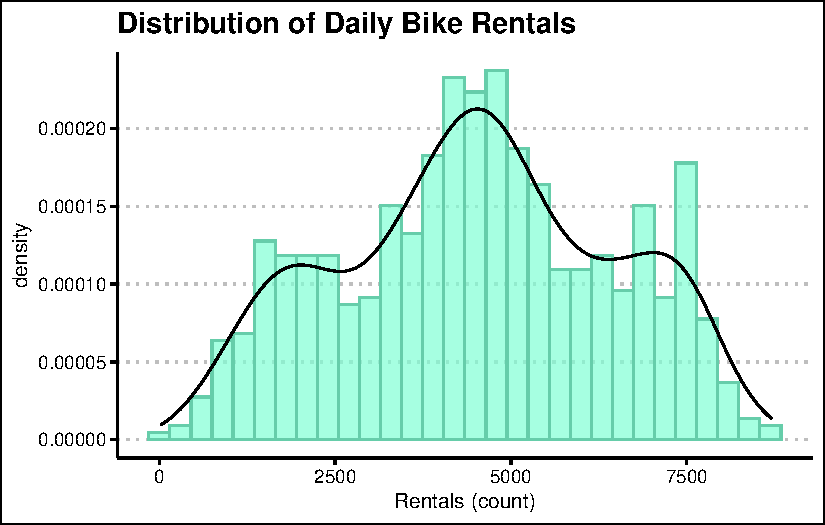
\includegraphics{index_files/figure-pdf/unnamed-chunk-12-1.pdf}

}

\end{figure}

Fortunately, we don't seem to have a huge number of outliers and the
distribution is not highly skewed. This means that we might not need to
make a log-transformation of this feature to make it more normal.
However, one thing to note is that it is a tri-model looking
distribution. There are peaks in the data which suggest that there might
be three different over-lapping normal distributions. A low, middle, and
high one.

\hypertarget{step-5}{%
\subsection{Step 5}\label{step-5}}

Many of the supervised learning algorithms can be helped or hurt by the
relationships between features that will be used as predictors. We need
to understand the distributions of each variable, looking for skew,
outliers, and any other weirdness. This could involve histograms or
boxplots of the variables. We can use scatter plots to look at
relationships between predictors. For easier comparison we can also use
correlation matrices to show statistically linear relationships.

\begin{Shaded}
\begin{Highlighting}[]
\NormalTok{bikes }\SpecialCharTok{\%\textgreater{}\%}
  \FunctionTok{keep}\NormalTok{(is.numeric) }\SpecialCharTok{\%\textgreater{}\%}
  \FunctionTok{ggpairs}\NormalTok{()}
\end{Highlighting}
\end{Shaded}

\begin{figure}[H]

{\centering 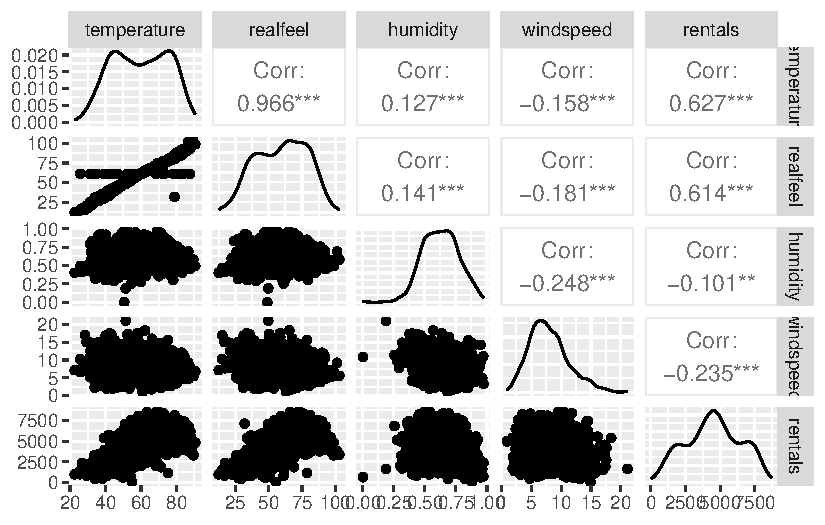
\includegraphics{index_files/figure-pdf/unnamed-chunk-13-1.pdf}

}

\end{figure}

First off we can see that \texttt{temperature} and \texttt{realfeel}
have an almost perfectly linear relationship. The correlation is 0.96!
This is a suspiciously strong relationship. In fact, this usually means
that one variable is a function of the other. Indeed, \texttt{realfeel}
is a relationship between temperature and humidity and wind that is mean
to incorporate what temperature \emph{it feels like to a human}. In such
a case, we will want to leave out a variable. Either \texttt{realfeel}
or the other features that go into it.

The distribution plots do not look particularly alarming. And the
scatterplots don't show any other overwhelmingly strong relationships.
What we can see, is that there is a positive and nonlinear relationship
between temperature and rentals. Warmer temps are associated with more
rentals (not surprising). But eventually, warmer temperatures result in
weather that is too hot for comfort - leading to decreased rentals.

We can also check these correlations with \texttt{corrplot}.

\begin{Shaded}
\begin{Highlighting}[]
\NormalTok{bikes }\SpecialCharTok{\%\textgreater{}\%}
  \FunctionTok{keep}\NormalTok{(is.numeric) }\SpecialCharTok{\%\textgreater{}\%}
  \FunctionTok{cor}\NormalTok{() }\SpecialCharTok{\%\textgreater{}\%}
  \FunctionTok{corrplot}\NormalTok{()}
\end{Highlighting}
\end{Shaded}

\begin{figure}[H]

{\centering 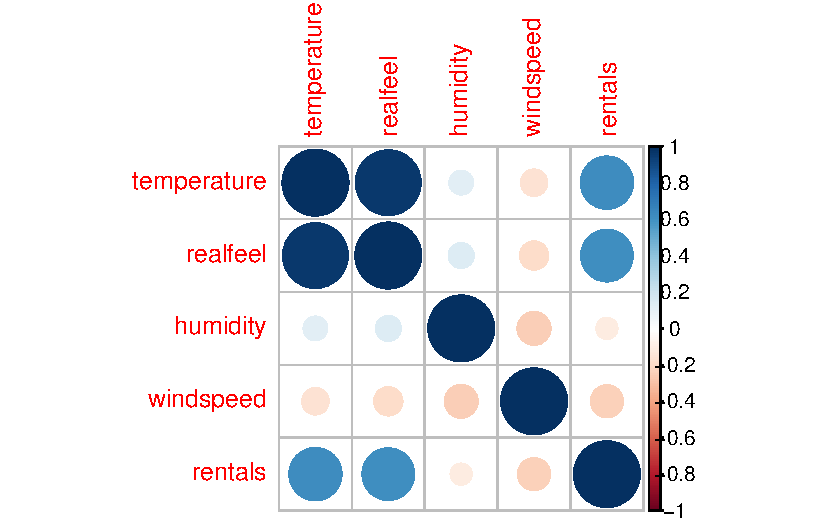
\includegraphics{index_files/figure-pdf/unnamed-chunk-14-1.pdf}

}

\end{figure}

Sometimes we need to convert features to achieve different objectives.

\begin{enumerate}
\def\labelenumi{\arabic{enumi}.}
\tightlist
\item
  We might transform a feature to make it easier for our learning
  algorithm to use, or
\item
  we might transform a feature to put it on the same or similar scale
  with the the other features.
\end{enumerate}

We're going to Z-score normalize the \texttt{temperature} feature. Our
reason is mostly arbitrary, but one benefit is that after the
transformation the mean will be zero. Positive numbers will represent
above average temperatures and negative below average ones.

\begin{Shaded}
\begin{Highlighting}[]
\NormalTok{bikes }\OtherTok{=}\NormalTok{ bikes }\SpecialCharTok{\%\textgreater{}\%}
  \FunctionTok{mutate}\NormalTok{(}\AttributeTok{temperature =}\NormalTok{ (temperature }\SpecialCharTok{{-}} \FunctionTok{mean}\NormalTok{(temperature))}\SpecialCharTok{/}\FunctionTok{sd}\NormalTok{(temperature))}

\NormalTok{bikes }\SpecialCharTok{\%\textgreater{}\%}
  \FunctionTok{select}\NormalTok{(temperature) }\SpecialCharTok{\%\textgreater{}\%}
  \FunctionTok{summary}\NormalTok{()}
\end{Highlighting}
\end{Shaded}

\begin{verbatim}
  temperature      
 Min.   :-2.38324  
 1st Qu.:-0.86479  
 Median : 0.01611  
 Mean   : 0.00000  
 3rd Qu.: 0.87425  
 Max.   : 2.00098  
\end{verbatim}

We can min-max normalize the wind variable. This will take all values of
the feature and cram it into the interval \([0, 1]\). It essentially
puts a feature into a percent range.

\begin{Shaded}
\begin{Highlighting}[]
\NormalTok{bikes }\OtherTok{=}\NormalTok{ bikes }\SpecialCharTok{\%\textgreater{}\%}
  \FunctionTok{mutate}\NormalTok{(}\AttributeTok{windspeed =}\NormalTok{ (windspeed }\SpecialCharTok{{-}} \FunctionTok{min}\NormalTok{(windspeed))}\SpecialCharTok{/}\NormalTok{(}\FunctionTok{max}\NormalTok{(windspeed)}\SpecialCharTok{{-}}\FunctionTok{min}\NormalTok{(windspeed)))}
\end{Highlighting}
\end{Shaded}

A very important step, and a very common one required by many learning
algorithms, is converting all categorical variables into dummy
variables. This can be done many different ways in R. The \texttt{dummy}
package does make it easier, however.

\begin{Shaded}
\begin{Highlighting}[]
\CommentTok{\# Convert every factor type feature into }
\CommentTok{\# a collection dummy variables.}
\NormalTok{bikes\_dummies }\OtherTok{=} \FunctionTok{dummy}\NormalTok{(bikes, }\AttributeTok{int =} \ConstantTok{TRUE}\NormalTok{)}
\end{Highlighting}
\end{Shaded}

Before running the \texttt{dummy()} function we had 10 variables in the
dataset. The result of the function is a new dataset with only the dummy
variables generated from the factor variables in \texttt{bikes}. At this
point we can replace the factor variables with the dummy ones.

\begin{Shaded}
\begin{Highlighting}[]
\NormalTok{bikes\_num }\OtherTok{=}\NormalTok{ bikes }\SpecialCharTok{\%\textgreater{}\%} \FunctionTok{keep}\NormalTok{(is.numeric)}
\NormalTok{bikes }\OtherTok{=} \FunctionTok{bind\_cols}\NormalTok{(bikes\_num, bikes\_dummies)}
\end{Highlighting}
\end{Shaded}

\hypertarget{step-6}{%
\subsection{Step 6}\label{step-6}}

We're going to perform a penalized form of regression known as LASSO to
find a decent predictive model. We'll need to do a few things first. We
need to get rid variables we don't intend to have as predictors. The
\texttt{date} and \texttt{realfeel} features will be removed.

\begin{Shaded}
\begin{Highlighting}[]
\NormalTok{bikes }\OtherTok{=}\NormalTok{ bikes }\SpecialCharTok{\%\textgreater{}\%}
  \FunctionTok{select}\NormalTok{(}\SpecialCharTok{{-}}\NormalTok{realfeel) }\SpecialCharTok{\%\textgreater{}\%}
  \FunctionTok{mutate}\NormalTok{(}\AttributeTok{temperature2 =}\NormalTok{ temperature}\SpecialCharTok{\^{}}\DecValTok{2}\NormalTok{)}
\end{Highlighting}
\end{Shaded}

Normally, for a linear regression, you'd need to remove one dummy
variable from a categorical variable. For example, season has 4 values
(Winter, Spring, Fall, and Summer). We have dummy variable for each, but
we need to omit one in order for it to work. But with LASSO, its okay
and actually better to include them all and let the algorithm decide
which to eliminate.

\begin{Shaded}
\begin{Highlighting}[]
\CommentTok{\# Separate predictors from target feature.}
\NormalTok{rentals }\OtherTok{=}\NormalTok{ bikes}\SpecialCharTok{$}\NormalTok{rentals}
\NormalTok{predictors }\OtherTok{=} \FunctionTok{as.matrix}\NormalTok{(}\FunctionTok{select}\NormalTok{(bikes, }\SpecialCharTok{{-}}\NormalTok{rentals))}
  

\CommentTok{\# estimate model}
\NormalTok{cv.model }\OtherTok{=}\NormalTok{ gamlr}\SpecialCharTok{::}\FunctionTok{cv.gamlr}\NormalTok{(}\AttributeTok{x=}\NormalTok{predictors, }\AttributeTok{y=}\NormalTok{rentals)}
\end{Highlighting}
\end{Shaded}

\begin{verbatim}
Loading required package: gamlr
\end{verbatim}

\begin{verbatim}
Loading required package: Matrix
\end{verbatim}

\begin{verbatim}

Attaching package: 'Matrix'
\end{verbatim}

\begin{verbatim}
The following objects are masked from 'package:tidyr':

    expand, pack, unpack
\end{verbatim}

\begin{Shaded}
\begin{Highlighting}[]
\FunctionTok{plot}\NormalTok{(cv.model)}
\end{Highlighting}
\end{Shaded}

\begin{figure}[H]

{\centering 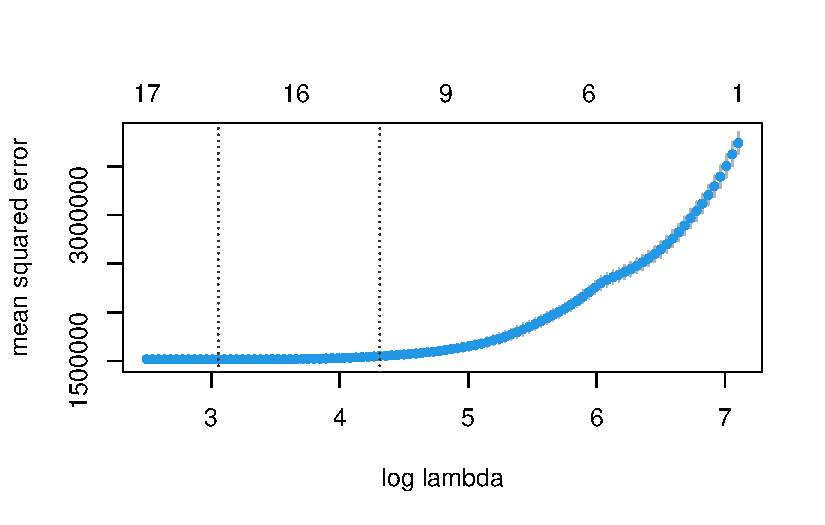
\includegraphics{index_files/figure-pdf/unnamed-chunk-20-1.pdf}

}

\end{figure}

\begin{Shaded}
\begin{Highlighting}[]
\NormalTok{betamin }\OtherTok{=} \FunctionTok{coef}\NormalTok{(cv.model, }\AttributeTok{select =} \StringTok{"min"}\NormalTok{)}
\NormalTok{betamin}
\end{Highlighting}
\end{Shaded}

\begin{verbatim}
21 x 1 sparse Matrix of class "dgCMatrix"
                    seg88
intercept      7164.94628
temperature     976.24016
humidity      -2958.56546
windspeed     -1846.32168
season_Winter  -724.33128
season_Spring   -85.88183
season_Summer    11.02263
season_Fall     299.97692
holiday_0       424.40407
holiday_1         .      
weekday_0      -250.94142
weekday_1       -88.67330
weekday_2         .      
weekday_3         .      
weekday_4         .      
weekday_5         .      
weekday_6        54.80502
weather_1       255.65491
weather_2         .      
weather_3     -1646.70892
temperature2   -524.66919
\end{verbatim}

\begin{Shaded}
\begin{Highlighting}[]
\NormalTok{bikes }\OtherTok{=}\NormalTok{ bikes }\SpecialCharTok{\%\textgreater{}\%}
  \FunctionTok{mutate}\NormalTok{(}\AttributeTok{pred =} \FunctionTok{as.numeric}\NormalTok{(}\FunctionTok{predict}\NormalTok{(cv.model, predictors)))}
\end{Highlighting}
\end{Shaded}

\begin{Shaded}
\begin{Highlighting}[]
\NormalTok{bikes }\SpecialCharTok{\%\textgreater{}\%}
  \FunctionTok{ggplot}\NormalTok{(}\FunctionTok{aes}\NormalTok{(}\AttributeTok{x=}\NormalTok{rentals, }\AttributeTok{y=}\NormalTok{pred)) }\SpecialCharTok{+}
  \FunctionTok{geom\_point}\NormalTok{()}
\end{Highlighting}
\end{Shaded}

\begin{figure}[H]

{\centering 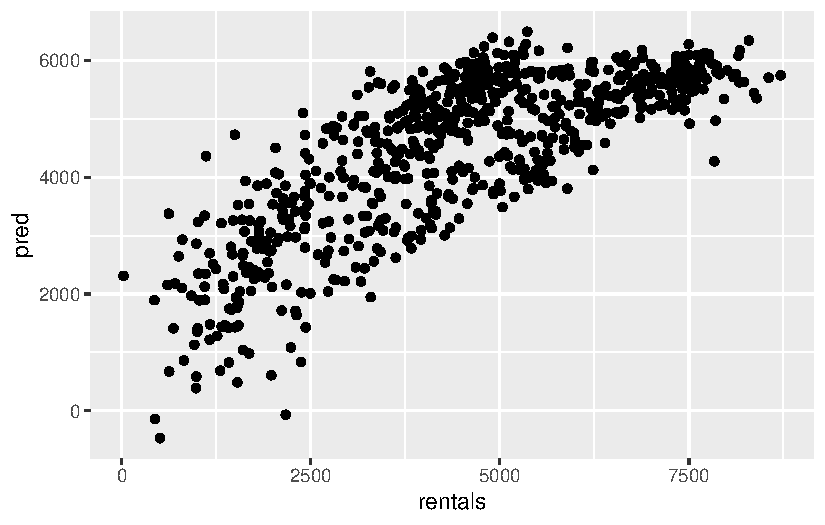
\includegraphics{index_files/figure-pdf/unnamed-chunk-23-1.pdf}

}

\end{figure}



\end{document}
